\documentclass[a4paper, 12pt]{article}

\newcommand{\templates}{../../template}
\usepackage[a4paper, margin=2.5cm]{geometry}

\usepackage{enumitem}
\setlist[itemize]{noitemsep}
\setlist[enumerate]{noitemsep}

\let\oldpar\paragraph
\renewcommand{\paragraph}[1]{\oldpar{#1\\}\noindent}
\usepackage{graphicx}
\usepackage{hyperref}
\usepackage{makecell}

\newcommand{\settitolo}[1]{\newcommand{\titolo}{#1\\}}
\newcommand{\setprogetto}[1]{\newcommand{\progetto}{#1\\}}
\newcommand{\setcommittenti}[1]{\newcommand{\committenti}{#1\\}}
\newcommand{\setredattori}[1]{\newcommand{\redattori}{#1\\}}
\newcommand{\setrevisori}[1]{\newcommand{\revisori}{#1\\}}
\newcommand{\setresponsabili}[1]{\newcommand{\responsabili}{#1\\}}
\newcommand{\setversione}[1]{
	\ifdefined\versione\renewcommand{\versione}{#1\\}
	\else\newcommand{\versione}{#1\\}\fi
}
\newcommand{\setdestuso}[1]{\newcommand{\uso}{#1\\}}
\newcommand{\setdescrizione}[1]{\newcommand{\descrizione}{#1\\}}

\newcommand{\makefrontpage}{
	\begin{titlepage}
		\begin{center}

		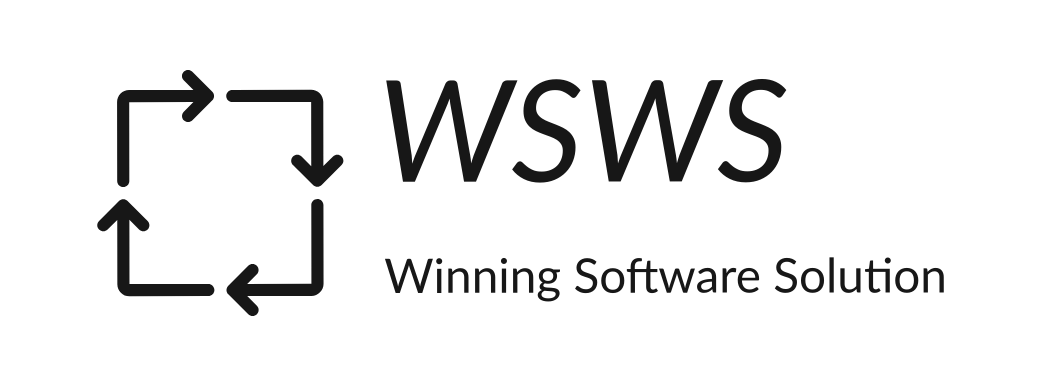
\includegraphics[width=0.4\textwidth]{../../template/WSWS-logos_transparent_crop}\\

		{\Large Winning Software Solution}\\[6pt]
		\href{mailto://winningsoftwaresolution@gmail.com}{winningsoftwaresolution@gmail.com}\\
		
		\ifdefined\progetto
		\vspace{1cm}
		{\Large\progetto}
		{\large\committenti}
		\else\fi
		
		\vspace{1.5cm}
		{\LARGE\titolo}
		
		\vfill
		
		\begin{tabular}{r | l}
		\multicolumn{2}{c}{\textit{Informazioni}}\\
		\hline
		
		\ifdefined\redattori
			\textit{Redattori} &
			\makecell[l]{\redattori}\\
		\else\fi
		\ifdefined\revisori
			\textit{Revisori} &
			\makecell[l]{\revisori}\\
		\else\fi
		\ifdefined\responsabili
			\textit{Respondabili} &
			\makecell[l]{\responsabili}\\
		\else\fi
		
		\ifdefined\versione
			\textit{Versione} & \versione
		\else\fi
		
		\textit{Uso} & \uso
		
		\end{tabular}
		
		\vspace{2cm}
		
		\ifdefined\descrizione
		Descrizione
		\vspace{6pt}
		\hrule
		\descrizione
		\else\fi
		\end{center}
	\end{titlepage}
}
\usepackage{hyperref}
\usepackage{array}
\usepackage{tabularx}

\def\vers#1-#2-#3-#4-#5\\{#1&#2&#3&#4&#5\\\hline}

\newcommand{\addversione}[5]{
	\ifdefined\versioni
		\let\old\versioni
		\renewcommand{\versioni}{#1&#2&#3&#4&#5\\\hline\old}
	\else
		\newcommand{\versioni}{#1&#2&#3&#4&#5\\\hline}
	\fi
}

\newcommand{\setversioni}[1]{\newcommand{\versioni}{#1}}

\newcommand{\makeversioni}{
	\begin{center}
		\begin{tabularx}{\textwidth}{|c|c|c|c|X|}
		\hline
		\textbf{Versione} & \textbf{Data} & \textbf{Persona} & \textbf{Attivtà} & \textbf{Descrizione} \\
		\hline
		\versioni
		\end{tabularx}
	\end{center}
	\clearpage
}

%package
\usepackage[table,xcdraw]{xcolor}

\settitolo{Relazione sull'architettura del progetto}
\setredattori{Matteo Galvagni}
\setdestuso{esterno}
\setdescrizione{
Relazione sull'architettura del progetto.
}

\begin{document}

\makefrontpage

\section{Il problema}

\subsection*{Premesse}
Tra le possibili soluzioni proposte dal gruppo di lavoro, la più promettente permetteva di effettuare la "validazione" delle transazioni (controllare che il denaro inviato corrispondesse a quello in attesa di ricezione) lato blockchain: il venditore avrebbe dovuto, durante la messa in vendita dei prodotti, firmare una transazione che includesse il prezzo atteso per quel prodotto direttamente in blockchain, in modo tale che all'arrivo di denaro si potesse controllare direttamente dal contratto la correttezza di un pagamento; dalla blockchain, invece, sarebbe stato generato un ID univoco per ogni istanza di pagamento \textit{valida}
che sarebbe servito a collegare ordine e pagamento. Ogni cliente, invece, avrebbe pagato tramite una transazione una certa istanza di pagamento dato il suo ID, transazione che sarebbe stata automaticamente rigettata
in caso di importo errato. Questa soluzione, seppur funzionante, è poco comoda per un venditore che dovrebbe firmare una transazione per ogni prodotto in vendita manualmente, il chè implica che per un buon funzionamento del metodo di pagamento sarebbe necessario uno script lato venditore per la messa in vendita in automatico dei prodotti, andando a modificare parte del backend dell'ecommerce.
Da qui in poi ci riferiremo a questa modalità come la "prima" soluzione.\\\\
Dal colloquio del 22/12 con la Proponente è emersa una nuova possibile architettura del progetto che mira a risolvere il problema della modifica del backend da parte dei venditori eliminando, almeno dal punto di vista teorico, questa necessità.
Questa soluzione prevede che alla messa in vendita di un oggetto non vi sia alcuna interazione con la blockchain da parte del venditore: tali interazioni dovrebbero verificarsi solo al momento dell'acquisto da
parte dei clienti. È previsto che l'ecommerce, al momento della richiesta del nostro servizio di pagamento, comunichi il suo ID interno dell'ordine in modo tale che il cliente possa firmare una transazione (tramite la nostra landing page) che includa tale ID, inviando inoltre il denaro richiesto. Alla ricezione della transazione, lato blockchain, il nostro server sarebbe in costante ascolto per notificare il venditore.
L'idea maturata è che il venditore abbia a disposizione una pagina dove visualizzare le transazioni in entrata e con la possibilità di annullarle qualora ritenesse il prezzo pagato errato, eliminando la
necessità di uno script lato venditore. D'ora in poi ci riferiremo a questa modalità come la "seconda" soluzione.

\newpage

\subsection*{Le perplessità}
Assumendo l'inesistenza di uno script lato venditore/ecommerce (per garantire la non modifica del backend come da seconda soluzione) e analizzando a fondo questa soluzione sono stati rilevati potenziali problemi tali che, nonostante risolvibili, le loro soluzioni appaiono scomode e/o controproducenti sia per i venditori sia per i clienti.
Di seguito una lista di problemi con possibili soluzioni.

\begin{itemize}
\item \textbf{Insicurezza sulla validità delle transazioni lato blockchain}
Ogni qualvolta arrivi una transazione di un cliente in blockchain a lato contratto digitale non è possibile sapere se tale transazione contenga il denaro atteso dal venditore o meno.
Vi è un'insicurezza su cosa il contratto dovrebbe fare quando del denaro è inviato: se, lato contratto, assumiamo che la transazione andrà a buon fine e sarà validata dal venditore (non accettando quindi altre transazioni per lo stesso ID ordine) il venditore perderebbe un considerevole ammontare di tempo in cui l'oggetto è in vendita in caso la transazione sia truffaldina, in quanto durante tutto il tempo in cui il venditore o chi per esso non possa approvare o annullare la transazione (fuori orario lavorativo, ferie, malattia...) l'oggetto non sarebbe più disponibile; se d'altro canto non facciamo questo tipo di controllo,
nel tempo sopracitato in cui una transazione non potrà essere annullata o confermata a lato venditore più clienti potrebbero comprare e pagare correttamente lo stesso oggetto, per poi vedersi la transazione annullata
apparentemente senza motivo ore o nei casi peggiori giorni dopo.\\

\item \textbf{Scomodità per il venditore}
Accettare o annullare transazioni manualmente è oggettivamente scomodo per il venditore, ed inoltre è lo stesso problema che è stato riscontrato nella prima soluzione dove è stato detto che approvare manualmente
le transazioni nella messa in vendita è inaccettabile per un grande ecommerce.\\

\item \textbf{Più transazioni richieste per il venditore}
Vi sono essenzialmente tre modi per approvare o annullare una transazione lato venditore.
Il primo necessita della sola operazione di annullamento di transazione, ma necessita invece di un timer oltre la quale se una transazione non è annullata viene considerata approvata automaticamente in modo da poter notificare il cliente che l'ordine è andato a buon fine; il secondo necessita di due operazioni diverse (approvazione e annullamento di transazione) e non necessita invece di un timer; il terzo prevede l'esistenza di una funzione di approvazione delle transazioni e non di quella di annullamento (con eventualmente un timer di annullamento per transazioni in \textit{pending} da troppo tempo).
Con la prima modalità vi è un problema di tempistiche: il timer dovrebbe essere abbastanza ampio da coprire eventuali mancanze umane, probabilmente nell'ordine delle ore, senza contare che fuori orario lavorativo ogni transazione non annullata verrebbe considerata valida a meno di avere un dipendente sempre presente per annullare le transazioni o di avere un timer nell'ordine dei giorni (con conseguente notifica al cliente di avvenuto ordine dopo giorni), entrambe soluzioni estremamente scomode o per il venditore o per i clienti.
\newpage
Con la seconda modalità, invece, vi è un problema sul numero delle transazioni che un venditore dovrebbe eseguire: mentre con la prima soluzione è possibile mettere in vendita N unità di uno stesso oggetto in una sola transazione, nella seconda soluzione con questa modalità N + Z transazioni sarebbero richieste per approvare N transazioni dei clienti e annullare Z transazioni con importi non corretti.
Questo significa che, nel migliore dei casi (nessuna transazione truffaldina) serviranno almeno N transazioni per approvare N acquisti, eventualità che nella prima soluzione si verifica solo nel caso peggiore (N oggetti \textit{unici} da mettere in vendita).
Sulla seconda modalità vi è un'altra perplessità: avendo il venditore piena autonomia nel confermare o annullare le transazioni, e avendo i clienti piena capacità di inserire un qualsiasi importo nella transazione senza essere rigettati o approvati lato blockchain, la logica della vendita di un prodotto si può spostare da vendita a prezzo fisso ad asta online. Un venditore potrebbe essere incentivato a non approvare una transazione oggettivamente valida in attesa di altre transazioni eventualmente di importo maggiore, per poi approvare una di esse. Questo è un caso estremo in quanto prevede un decente numero di clienti consapevoli del funzionamento di una transazione in blockchain e con le capacità di crearne una e inviarla autonomamente, ma riteniamo che sia utile citare comunque tutto ciò come perplessità (non come problema, in quanto rappresenta un vantaggio per il venditore ma uno svantaggio per i clienti che non conoscono il funzionamento interno delle transazioni) che potrebbe modificare la logica della vendita in caso di alta domanda di un bene.
\\\\Con la terza e ultima modalità il venditore dovrebbe solo approvare le transazioni che ritiene valide, mentre le altre sarebbero automaticamenta annullate lato blockchain. Questa modalità conserva la perplessità della seconda modalità sul cambio di logica della vendita e, anche se risolve parte della problematica sul numero di transazioni (N transazioni per approvare N vendite e non N + Z, anche se è solo il caso \textit{peggiore} della prima soluzione), introduce un problema di inefficienza: una volta approvata una transazione, lato blockchain sarebbe necessario scorrere tutta la lista di transazioni per annullare tutte le altre transazioni con ID ordine uguale a quella approvata (complessità O(n)). Se, invece, utilizzassimo un ID numerico crescente generato lato blockchain per identificare le transazioni (invece dell'ID ordine interno degli ecommerce) dovremmo salvare o sul nostro database o su quello dell'ecommerce tutti gli ID di ogni transazione per un certo oggetto, in modo da sapere quali annullare ricercandoli lato blockchain con complessità O(nlogn), ma il salvataggio di questi ID introdurrebbe molte più letture e scritture su database nonchè uno spreco di spazio non indifferente.
Inoltre vi è lo stesso problema di tempistica della prima modalità: fuori orario lavorativo tutte le transazioni rimarrebbero in stallo per ore in attesa di essere approvate o annullate automaticamente il giorno seguente, a meno dell'utilizzo di un timer (che però renderebbe impossibile la vendita online fuori orario lavorativo).

\end{itemize}

\newpage

\subsection*{Possibile soluzione}
La soluzione più ovvia per risolvere quantomeno i problemi sopracitati riguardanti le tempistiche sarebbe utilizzare uno script lato venditore che approva o annulla automanticamente le transazioni, ma questo va direttamente contro la ragione per la quale questa soluzione è stata pensata in primo luogo. Inoltre, anche con uno script, verrebbero conservati alcuni problemi (per esempio il numero di transazioni richieste), senza contare la responsabilità enorme da parte del venditore che implicherebbe: lo script per un qualche errore di progettazione potrebbe accettare transazioni di importo diverso, dunque la corretta progettazione di tale script sarebbe di importanza fondamentale; lo script, se smettesse di funzionare per un qualsiasi motivo (bug, server down...), non potrebbe più accettare o annullare le transazioni in entrata che, nel migliore dei casi (terza modalità di approvazione, senza timer) farebbe rimanere transazioni in stallo per ore o giorni, mentre nel peggiore dei casi (prima modalità) passato il tempo del timer ogni transazione non annullata sarebbe approvata anche se scorretta.
\\\\Dopo un'analisi di questo tipo di soluzione ci è chiaro che l'unico modo in cui potrebbe funzionare sarebbe con uno script lato venditore, e non risolverebbe comunque tutti i problemi ma solo una parte, aggiungendo una responsabilità e un lavoro in più da parte del venditore che potrebbe disincentivarlo da utilizzare il nostro servizio a favore dell'utilizzo di un servizio più comodo e pratico.

\newpage

\section{Soluzione proposta}
A seguito di una discussione all'interno del gruppo riteniamo che adottare la seconda soluzione, seppur funzionante, introdurrebbe più problematiche di quante ne possa risolvere.
Essendo uno script lato venditore che interagisce con la blockchain comunque necessario (per la vendita automatica o l'approvazione automatica delle transazioni) sia nella prima soluzione che nella seconda, dunque a parità di problema, troviamo che la prima soluzione sia più adatta ad essere adottata come architettura per questo progetto: tutte le perplessità e problematiche sopracitate non sono presenti nella prima soluzione in quanto a lato blockchain è conosciuto l'importo dovuto e le validazioni possono essere effettuate direttamente dal contratto in modo automatico e al momento esatto dell'acquisto non lasciando spazi a possibili ritardi temporali o richieste di personale eccessive per i venditori.
Inoltre, il contratto digitale risultante dalla scelta della prima soluzione sarebbe abbastanza generalizzato da funzionare sia su ecommerce di vendita diretta (con script per la messa in vendita automatica) sia su ecommerce di vendita tra privati (senza necessità di script), ampliando il bacino d'utenza possibile per questo progetto.\\\\
Nonostante ciò ci è chiaro come sia sconveniente (anche se purtroppo necessaria) la presenza di uno script lato backend per i venditori.
È per questo che, con il permesso della Proponente, suggeriamo di sviluppare il progetto secondo la prima architettura descritta \textit{nonchè} lo script che dovrà occuparsi della messa in vendita automatica degli oggetti, in modo tale che un venditore che volesse utilizzare il nostro metodo di pagamento sia quanto più facilitato possibile e in modo che la firma delle transazioni e la creazione dell'istanza di pagamento in blockchain sia "nascosta" e non richieda l'utilizzo di Metamask, ma solo che il venditore segua il normale iter di messa in vendita degli oggetti.

\end{document}
